\documentclass[11pt,a4paper]{article}
\usepackage[utf8]{inputenc}
\usepackage[T1]{fontenc}
\usepackage{lmodern}
\usepackage[margin=25mm]{geometry}
\usepackage{amsmath,amssymb,graphicx,booktabs,longtable,array,microtype}
\usepackage[hidelinks]{hyperref}
\graphicspath{{../../product-report/figures/}}
\setlength{\parindent}{0pt}
\setlength{\parskip}{5pt}
\setlength{\LTcapwidth}{\textwidth}
\newcommand{\doctype}{Preprint}
\newcommand{\docversion}{v0.2}
\newcommand{\docdate}{2 November 2026}
\newcommand{\versiondoi}{10.5281/zenodo.23884371}
\newcommand{\conceptdoi}{10.5281/zenodo.23874820}
\newcommand{\docrepo}{github.com/fsantibanezleal/CAOS\_RES\_ChronoScope}
\newcommand{\headerblock}{\begin{center}\fbox{\parbox{0.94\textwidth}{\small\raggedright
\textbf{\doctype}\quad \docversion, \docdate\quad Licence CC BY 4.0\\[2pt]
CAOS open-research programme; ChronoScope context-dependent forecasting.\\[2pt]
Version DOI: \versiondoi. Concept DOI (always latest): \conceptdoi.\\[2pt]
Not peer reviewed. Source, inputs and computational records: \url{https://github.com/fsantibanezleal/CAOS_RES_ChronoScope}.
}}\end{center}}
\title{Forecast Combination with Temporal Validation and Context Memory}
\author{Felipe Santib\'a\~nez-Leal\\CAOS open-research programme, Santiago, Chile\\\small ORCID: 0000-0002-0150-3246}
\date{}
\hypersetup{pdftitle={Forecast Combination with Temporal Validation and Context Memory},pdfauthor={Felipe Santibáñez-Leal}}
\begin{document}
\maketitle
\headerblock
\begin{abstract}
A forecast combination must decide how much historical expert performance remains relevant at a new origin. We study a fixed context-weighted rule and two variants that select their parameters using completed historical target blocks. ContextMemoryCV selects context shrinkage and temperature; ValidationMix also considers regularized convex stacking. Each inner fit excludes outcomes not yet observed at its validation origin. The original fifteen-case experiment remains negative for fixed ContextMemory, with mean MASE 1.4504 versus 1.4489 for its recency-only ablation. In a separate external evaluation, 294 of 359 M4 Weekly series satisfy the fixed history criterion, and 1,422 of 1,428 M3 Monthly series remain after exact deduplication. ValidationMix has mean series MASE 0.2855 versus 0.3109 for RecencyMean on M4 Weekly, and 0.8993 versus 0.9085 on M3 Monthly. AutoTheta gives 0.3076 and 0.8472, respectively: improvement over the recency control does not establish superiority on both collections. Interval scores also retain unfavorable outcomes. Full forecast paths, scales, weights, validation decisions and source hashes support independent recomputation of 53,148 external forecasts. These results concern the configured algorithms and admitted series; they neither establish priority for context weighting nor prove population-wide superiority or calibrated uncertainty.
\end{abstract}

\section{Question and relation to prior work}
Combining forecasters can reduce dependence on one modelling assumption, but estimated expert weights can introduce another source of error. When a series changes regime, a recent expert loss may be more relevant than a long-run average. When an earlier regime recurs, a remembered context may instead carry useful information. The concrete question is whether a small context-distance weighting rule improves a combination beyond an otherwise matching recency-only estimate.

Feature-based forecast averaging and dynamic expert arbitration already address context-dependent combinations. FFORMA learns a feature-to-weight mapping across a collection of reference series~\cite{fforma}. Arbitrated dynamic ensembles learn and combine expert-competence estimates~\cite{ade}. These precedents prevent interpreting the existence of contextual weighting as a new general idea. The proposed experiment concerns one particular low-data, within-series memory construction. A small implementation and matching ablations make its mechanism falsifiable; they do not establish priority over earlier ensemble research.

The primary comparison is mean final-block MASE of ContextMemory against RecencyMean over all fifteen selected cases. Configuration values are fixed in the released implementation; this is a retrospective experiment, not a prospectively registered trial or an independently selected confirmation corpus. An unfavorable mean difference provides no aggregate benefit in this experiment. It does not establish that every possible contextual rule is ineffective. Individual case outcomes, interval width and empirical coverage remain visible so that a favorable subset cannot replace the aggregate question.

\section{Information available at an origin}
Let the observed prefix be $y_{1:n}$, the forecast horizon be $H$ and the seasonal lag be $m$. The final targets $a_{1:H}$ are used only for evaluation. Historical training origins belong to
\begin{equation}
\mathcal O\subseteq\{o:o\geq o_{\min},\quad o+H\leq n\},
\qquad o_{\min}=\max(2m,2H+8,24).
\end{equation}
At most twelve distinct origins are selected as the unique integer values of a twelve-point equally spaced grid from $o_{\min}$ to $n-H$, with nonnegative grid values truncated to integers. An empty eligible interval supplies no memory. Every expert at origin $o$ receives $y_{1:o}$, and its loss uses $y_{o+1:o+H}$. The requirement $o+H\leq n$ ensures that all remembered targets have arrived before the final query. An origin near the end of the prefix is not eligible merely because its first future target is known; its complete scored horizon must be known.

The selection does not consume the final test block. Generated source definitions and admitted real-data CSVs reconstruct the original equally spaced histories. Every available released display sample is checked at its original time index, the original prefix length is verified, and the reserved targets are checked to their released four-decimal tolerance. A display-decimated replay array is explicitly rejected as a consecutive fitting sequence. This is necessary because changing observation spacing changes both context statistics and the seasonal error scale.

\section{Experts and contextual memory}
The fixed expert set is SeasonalNaive, SES, Holt, additive HoltWinters and nonseasonal finite-history Theta. Their parameter grids and Gaussian residual quantile rules belong to the implementation. They are shared unchanged by the proposal and both ablations. Seasonal continuation respects an incomplete terminal cycle; Theta includes the finite-history SES correction~\cite{theta}. No expert is removed after observing its final-block error.

The context uses recent and preceding windows of length $w=\min(\lfloor n/2\rfloor,\max(8,\min(2m,48)))$. Let $R=y_{n-w+1:n}$ and $P=y_{n-2w+1:n-w}$, let $s$ be the population standard deviation of their concatenation, and set $d=\lfloor w/2\rfloor$. For $w\ge2$ and $s\ge10^{-12}$, the first three features are
\begin{align}
f_1&=(\overline{R_{w-d+1:w}}-\overline{R_{1:d}})/s,\\
f_2&=(\overline R-\overline P)/s,\\
f_3&=\log\{(\operatorname{sd}(\Delta R)+10^{-6}s)/(\operatorname{sd}(\Delta P)+10^{-6}s)\}.
\end{align}
The first is a half-window mean contrast, not an OLS slope. The fourth is the Pearson correlation of the last two length-$m$ cycles when $m\ge2$, $n\ge2m+2$ and both cycle standard deviations exceed $10^{-12}$; otherwise it is zero. Every feature is clipped to $[-4,4]$. If the length or scale condition fails, all four features are zero. Population standard deviations use divisor equal to sample length.

For each remembered origin $o$ and expert $k$, the competence target is a normalized multi-step absolute loss
\begin{equation}
L_{ok}=\frac{H^{-1}\sum_{j=1}^H|y_{o+j}-p_{okj}|}{s_o},
\end{equation}
Here $s_o$ is the mean absolute lag-$m\prime$ difference in the prefix, with $m\prime=\max(1,\min(m,o-1))$. If that mean is at most $10^{-12}$, the training-loss scale is $\max(\operatorname{sd}(y_{1:o}),10^{-12})$. This training fallback differs from the final evaluation rule, which reports unavailable MASE for an exactly zero denominator. No scale is estimated from the final held-out block. The loss array and historical contexts are cached for a fitting history; caching changes runtime rather than the available information.

For remembered origins indexed $j=1,\ldots,J$, recency weights are $r_j=2^{-(J-j)/6}$. Distance to the query is $D_j=\sqrt{\frac14\sum_{a=1}^4(f_{ja}-f_{\mathrm{query},a})^2}$, bandwidth is $b=\max(\operatorname{median}_jD_j,.25)$, and local weights are $a_j=r_j\exp(-D_j^2/(2b^2))$. Expert competence is
\begin{equation}
c_k=.75\frac{\sum_j a_jL_{jk}}{\sum_j a_j}+.25\frac{\sum_j r_jL_{jk}}{\sum_j r_j}.
\end{equation}
Weights before the uniform floor are normalized values of $\exp(\max\{-(c_k-\min_lc_l),-700\})$. RecencyMean uses only the recency-weighted loss average, without context weighting or shrinkage. EqualMean, and any fit without remembered origins, uses $1/5$ directly. These settings are fixed; they are not retuned after inspecting the final blocks.

\subsection{Convexity and its limited consequence}
Let $v_k\geq0$ denote the normalized competence allocation before the uniform floor, so that $\sum_kv_k=1$. The final weight is
\begin{equation}
w_k=(1-\varepsilon)v_k+\frac{\varepsilon}{K},\qquad \varepsilon=0.05,\quad K=5.
\end{equation}
Thus $w_k\geq0.01$ and $\sum_kw_k=1$. If every input expert has ordered quantiles $q_{k,.1}\leq q_{k,.5}\leq q_{k,.9}$ at a lead, then
\begin{equation}
\sum_kw_kq_{k,.1}\leq\sum_kw_kq_{k,.5}\leq\sum_kw_kq_{k,.9}.
\end{equation}
This follows by multiplying each input inequality by a nonnegative weight and summing. It proves column order only. An average of marginal quantiles generally differs from the quantile function of a predictive mixture. No calibration or conditional-coverage guarantee follows from this construction.

The context features and normalized losses aim to make expert allocation insensitive to a positive change of units and a common level shift. The numerical implementation includes clipping and degeneracy thresholds, so structural invariance is tested away from those thresholds rather than claimed without qualification for every floating-point input. Independent tests also require finite paths, positive normalized weights and temporally complete historical targets.

\section{Matching ablations}
RecencyMean removes context-distance weighting and retains the experts, completed origins, recency decay and competence-to-weight transformation. It tests whether the contextual component adds value to an otherwise similar recent-loss combination. EqualMean removes estimated competence preferences and assigns a uniform allocation. All three compute their current expert paths from the same original prefix.

Comparing only with SeasonalNaive would not isolate the proposed mechanism: a gain might be due to combining experts rather than context similarity. Comparing only with EqualMean would similarly confound context with loss adaptation. The recency-only ablation is therefore the primary comparator. The equality of expert rosters, information sets and target blocks is part of the experimental contract, not a post hoc interpretation of whichever comparison is favorable.

\section{Evaluation protocol and invalidated calculation}
The corrected experiment uses fifteen selected cases, eleven generated and four real excerpts, with one final forecast origin per case. For the three combinations, all fitting paths are freshly computed. Other methods in the surrounding atlas include historical frozen forecasts and are not needed to isolate the context-versus-recency question. Their leaderboard positions do not substitute for the matching-expert ablation.

The first calculation incorrectly used display-decimated history arrays as consecutive inputs for nine cases. Its predictions, scales and aggregate values are invalidated. Reconstructing original histories fixes that defect. Every displayed observation matches its original indexed source within 0.000051, and the final targets also match. The invalidated artifact remains identifiable in Git so the correction is auditable; it is not pooled with the corrected experiment or counted as a replication.

The primary metric is MAE divided by the in-prefix mean absolute seasonal difference~\cite{mase}. This denominator is common to every final-block method within a case. It is not the error of a separately forecast future SeasonalNaive path. Zero denominators yield unavailable scaled metrics. Coverage and mean interval width are also retained. Three-quantile weighted loss and mean scaled interval score supply additional descriptive measures without implying an entire predictive distribution has been validated.

\section{Results}
\begin{longtable}{lrrr}
\caption{Matching-expert ablations: final-block MASE per selected case.}\\
\toprule Case & ContextMemory & RecencyMean & EqualMean\\\midrule\endhead
BRKV\_level\_shift & 0.7156 & 0.7313 & 0.8425\\
CHAO\_mackey & 1.8904 & 1.8923 & 1.9291\\
CTRL\_white\_noise & 1.0934 & 1.0754 & 1.1244\\
EXOG\_promo & 1.6955 & 1.7113 & 1.8232\\
HETV\_garch & 3.8878 & 3.9063 & 3.8056\\
INTM\_demand & 0.0938 & 0.0867 & 0.1132\\
LMEM\_fractional & 2.1341 & 2.1377 & 2.2060\\
MSEA\_daily\_weekly & 0.6951 & 0.6857 & 1.2424\\
REAL\_electricity & 0.6944 & 0.6937 & 0.7674\\
REAL\_m4\_daily & 0.2912 & 0.2939 & 0.2928\\
REAL\_m4\_hourly & 1.6003 & 1.6067 & 3.2852\\
REAL\_pm25 & 0.4174 & 0.4174 & 0.4173\\
RWLK\_noise & 4.9847 & 4.9333 & 5.0806\\
SEAS\_hourly & 1.0072 & 1.0070 & 4.4859\\
TRND\_seasonal & 0.5557 & 0.5545 & 1.0389\\
\midrule Mean & 1.4504 & 1.4489 & 1.8970\\
\bottomrule
\end{longtable}


\begin{figure}[htbp]\centering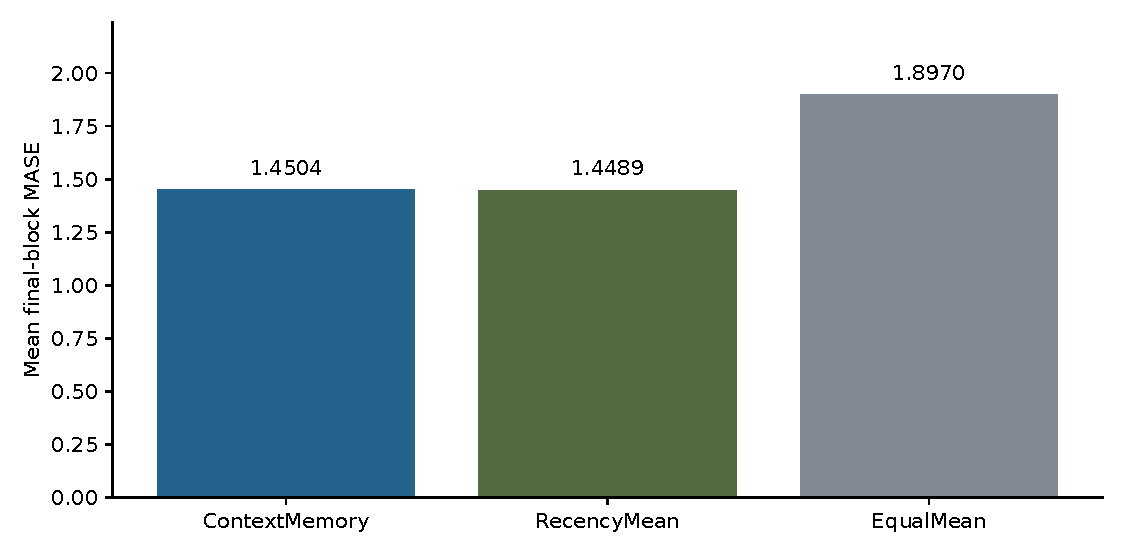
\includegraphics[width=0.88\textwidth]{proposal-comparison.pdf}
\caption{Mean MASE of the fixed combinations on all selected final blocks. ContextMemory is slightly worse than RecencyMean at the declared primary criterion. Bar heights are point summaries; no sampling uncertainty is shown because one selected origin per case does not supply a justified population interval.}\end{figure}

ContextMemory has mean MASE 1.4504, compared with 1.4489 for RecencyMean and 1.8970 for EqualMean. The contextual component fails its aggregate improvement criterion. The estimated recent-loss combinations perform better than the equal average on this collection, but that difference does not establish a benefit from the additional context kernel.

\begin{figure}[htbp]\centering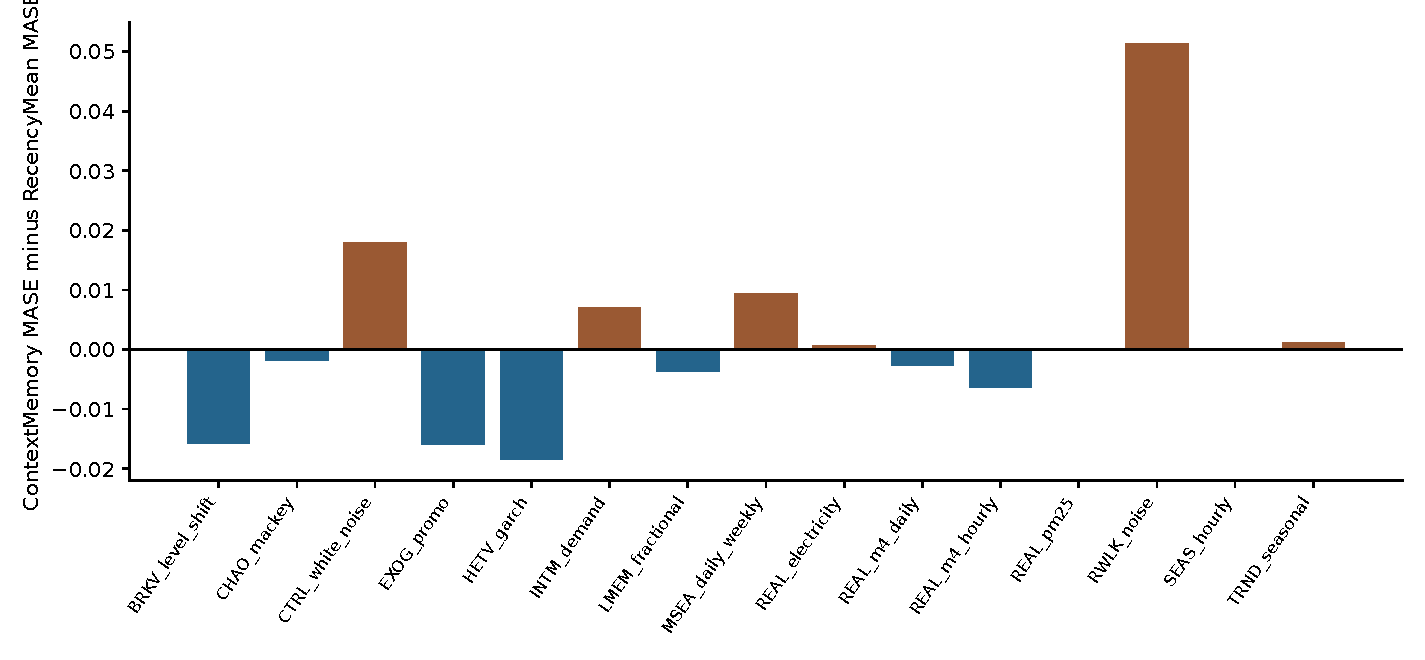
\includegraphics[width=\textwidth]{case-differences.pdf}
\caption{Per-case MASE difference between contextual and recency-only weighting. Each bar is one final block. Both signs are retained; selecting only negative bars would replace the declared aggregate question with a post hoc favorable subset.}\end{figure}

The aggregate difference is small relative to variation across selected mechanisms. It is still unfavorable at the criterion that was actually declared. Rounding both means to two decimal places would conceal that outcome. No significance claim, equivalence conclusion or general impossibility result is attached to the difference. Full-precision prediction paths and expert weights remain available so the cases that help and hurt can be inspected without reconstructing an aggregate from a selected table.

\section{Forecast combination with temporal validation}
The fixed context-versus-recency comparison tests one particular parameter setting. Two additional methods allow a historical validation calculation to choose a setting before an outer forecast. They retain the same five experts, four context features, completed-origin memory and quantile-column combination. Their improvements must not be attributed exclusively to the context kernel, because temperature, shrinkage and selection also change.

For every remembered validation origin $v$, only training origins $o$ satisfying $o+H\le v$ are eligible. At least three such origins are required. The candidate is fit on those completed earlier blocks, predicts the block beginning at $v$, and receives its mean absolute error divided by a scale calculated from the prefix at $v$. The final candidate score averages these eligible validation-block losses. The outer target is never an input to candidate fitting or selection. If no validation origin qualifies, the method uses the original RecencyMean rule.

ContextMemoryCV considers context shrinkages $\{0,.5,1\}$ and temperatures $\{.15,.5,1\}$, plus the original RecencyMean and EqualMean controls. Shrinkage one removes the context kernel, so selecting this method does not imply that contextual similarity helped. All settings retain recency half-life six, the original bandwidth rule and the 5\% uniform allocation floor. The first configured minimum wins an exact score tie. After selection, the chosen rule is fit on all completed memory blocks in the outer prefix.

ValidationMix additionally considers four convex stacking rules. Let $E_{jhk}=(p_{jhk}-y_{j+h})/s_j$ be expert $k$'s normalized error at completed training origin $j$ and lead $h$. For $\lambda\in\{.01,.1,1,10\}$, the unfloored stacking weights solve
\begin{equation}
\min_{w\ge0,\,\mathbf1^\top w=1}\frac{1}{JH}\sum_{j,h}\left(\sum_k E_{jhk}w_k\right)^2+\lambda\left\|w-\frac{\mathbf1}{5}\right\|_2^2.
\end{equation}
Five experts permit enumeration of the 31 nonempty active sets. Each face solves a regularized equality-constrained quadratic, and the feasible minimum is selected. A 5\% uniform floor is applied afterwards; the floored vector is not claimed to minimize the unfloored objective. Candidate selection still uses historical absolute error, rather than the squared fitting objective. The stacking family and its penalties are fixed before the external outcomes are computed. Neither established convex stacking nor temporal validation is claimed as a new general idea.

\section{External evaluation on weekly and monthly collections}
The sources are the complete Monash M4 Weekly inventory of 359 identities~\cite{weekly} and M3 Monthly inventory of 1,428 identities~\cite{monthly}, both redistributed under CC BY 4.0. ZIP, extracted TSF and exact sequence SHA-256 values identify their bytes. Forecast horizon and seasonal lag are $(13,52)$ for weekly and $(18,12)$ for monthly. Each series supplies up to three nonoverlapping final target blocks, provided that the prefix has at least $\max(2m,2H+8,24)$ observations. Every method receives the same final 512 contiguous prefix observations, or all observations if fewer are available. The scale uses this supplied prefix, and never the future block.

Sixty-five weekly identities have no eligible origin under that fixed criterion. All 294 eligible weekly series contribute three origins, giving 882 origins. Six exact duplicate monthly sequences retain one representative each; 1,422 monthly series contribute 3,547 eligible origins. Every exclusion and representative remains identifiable. Scores average origins within a series and then weight admitted series equally within each collection. The collections are reported separately; their different units, seasonal scales and origin counts are not silently pooled. This schedule and scaling differ from the original forecasting competitions, so the results do not establish an official competition rank.

Twelve methods are evaluated at every admitted origin: five individual experts, AutoETS and AutoTheta from StatsForecast, three fixed combinations, ContextMemoryCV and ValidationMix. Automatic statistical methods use the same available prefix and configured seasonal lag. Their library point forecast supplies the central column and their requested analytic 80\% interval supplies the endpoints. This roster contains no freshly evaluated neural, pretrained or globally trained ensemble on the external collections. A method failure stops the calculation rather than deleting a difficult comparator.

\begin{table}[htbp]\centering\small
\caption{Complete external comparison. W denotes 294 eligible M4 Weekly series; M denotes 1,422 unique M3 Monthly series. MASE and MSIS average origins within series and then series equally; Cov is empirical interval coverage. These are descriptive summaries, not confidence intervals.}
\begin{tabular}{lrrrrrr}\toprule Method & W MASE & W MSIS & W Cov & M MASE & M MSIS & M Cov\\\midrule
SeasonalNaive & 0.8446 & 8.1670 & 0.9326 & 1.0864 & 8.8123 & 0.9342\\
SES & 0.3533 & 2.3404 & 0.8926 & 1.0456 & 7.1945 & 0.8534\\
Holt & 0.3806 & 2.4611 & 0.8844 & 1.8040 & 10.8472 & 0.8005\\
HoltWinters & 0.5396 & 3.0778 & 0.8413 & 0.9375 & 6.7112 & 0.9160\\
Theta & 0.3469 & 2.3237 & 0.9041 & 1.0021 & 7.0453 & 0.8700\\
AutoETS & 0.3413 & 1.8490 & 0.8713 & 0.8514 & 4.1518 & 0.7324\\
AutoTheta & 0.3076 & 1.7125 & 0.8511 & 0.8472 & 4.2994 & 0.7279\\
ContextMemory & 0.3079 & 2.9468 & 0.9751 & 0.9086 & 6.8846 & 0.9348\\
RecencyMean & 0.3109 & 2.9315 & 0.9742 & 0.9085 & 6.8846 & 0.9348\\
EqualMean & 0.3548 & 3.3233 & 0.9702 & 0.9962 & 7.2131 & 0.9333\\
ContextMemoryCV & 0.2848 & 2.5538 & 0.9511 & 0.8996 & 6.7999 & 0.9329\\
ValidationMix & 0.2855 & 2.5477 & 0.9503 & 0.8993 & 6.8208 & 0.9326\\
\bottomrule\end{tabular}\end{table}

\begin{figure}[htbp]\centering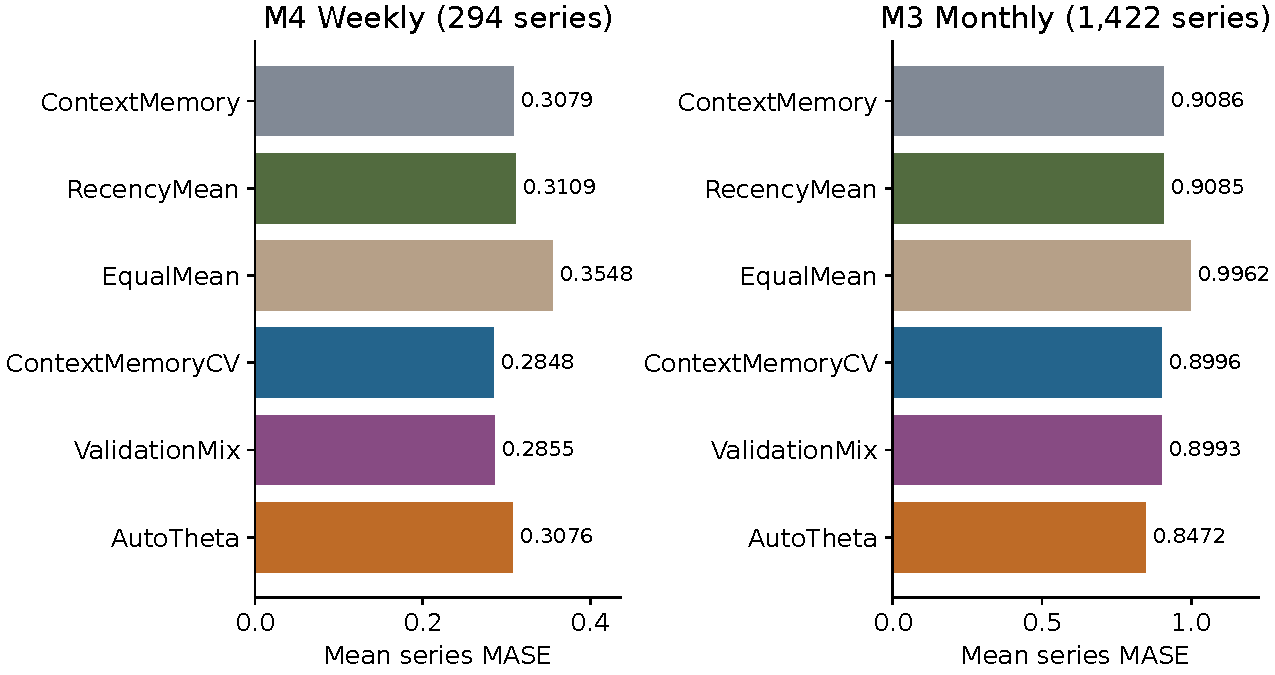
\includegraphics[width=.98\textwidth]{validated-combinations.pdf}
\caption{Fixed and temporally selected combinations alongside AutoTheta on each external collection. Bars are mean series MASE without sampling-error bars. The complete twelve-method table retains all individual-expert and automatic-statistical outcomes.}\end{figure}

ValidationMix has mean MASE .2855 versus .3109 for RecencyMean on weekly series, and .8993 versus .9085 on monthly series. ContextMemoryCV gives .2848 and .8996. AutoTheta gives .3076 and .8472: the temporally selected combinations have lower point error on the admitted weekly collection, while AutoTheta has lower point error on monthly series. These are finite-collection comparisons without an inferential or population-superiority claim.

Uncertainty quality does not follow the point-error ordering. ValidationMix has weekly MSIS 2.5477 and coverage .9503, versus AutoTheta's 1.7125 and .8511. On monthly series the corresponding values are 6.8208 and .9326, versus AutoTheta's 4.2994 and .7279. The combinations' wide Gaussian approximations remain a material limitation at nominal coverage .8. Selecting weights for point error does not calibrate their interval endpoints.

The original fifteen final blocks remain development examples. On those blocks ContextMemoryCV and ValidationMix have mean MASE 1.3974 and 1.4031; the original fixed contextual and recency-only results remain 1.4504 and 1.4489. Their MSIS values are 9.5025 and 9.3428 versus RecencyMean's 9.1076. The changed algorithms therefore improve this descriptive point score while worsening the interval score. Reusing these already examined cases is not independent external confirmation.

\section{Interpretation and limitations}
Context matching has a bias--variance tradeoff. A small within-series memory can contain few genuinely comparable contexts. Kernel weighting can overemphasize those few origins, while shrinkage and a uniform floor can dilute a useful specialist. A context can recur in its four descriptive statistics without recurring in the forecasting relationships that determine competence. The experiment does not identify which explanation caused the observed aggregate failure; that requires new controlled comparisons.

The original selected corpus and one final origin per series provide a bounded diagnostic experiment rather than representative population sampling. The additional weekly and monthly collections broaden empirical coverage, but eligibility exclusions, source relationships and limited rolling origins still constrain generalization. Training origins share observations and must not be counted as independent final-test replications. Methods also share experts and target series. A dependence-aware uncertainty analysis would need an explicitly designed repeated-origin or cross-series study. Neither the selected-case experiment nor the external collections support a superiority or equivalence statement for a deployment population.

Faithful external FFORMA and arbitrated-ensemble comparators remain necessary before asserting a research contribution beyond this tested construction. A fair study would also report fitting time, cache memory, inference latency and the information available to those comparators. A successful future experiment would not retroactively make this one successful. Any change to contexts, loss normalization, expert membership, shrinkage, bandwidth or the comparison collection must be named as a new configuration.

Quantile averaging and the experts' Gaussian approximations are further limits. An interval can achieve higher observed coverage by becoming too wide for useful planning. Evaluating an inventory action would require shortage and excess costs, decision lead times and prospective outcomes. Neither the generated examples nor real forecasting excerpts establish an operational benefit from this combination.

\section{Reproduction and conclusion}
Implementations and admitted numerical outputs are available in the \href{https://github.com/fsantibanezleal/CAOS_RES_ChronoScope/tree/d702831a7660f9fb8123798a2e3bbf5e47887bce}{frozen source and data snapshot}.

The fixed rule is implemented in \path{data-pipeline/chronoscopelab/model/context_memory.py}; the temporally validated variants are in \path{data-pipeline/chronoscopelab/model/validated_combination.py}. Tests check complete historical eligibility, deterministic selection, convex constraints, quantile order and the fallback identity. Recursive expert loops are optionally compiled with Numba without fast-math transformations; independent reference comparisons protect their forecast equations.

The external runner accepts explicit source, cache and output directories. Its cache binds source bytes, protocol, implementations and package versions. The full compressed numerical file is \path{manuscripts/context-memory/evidence/external-evaluation.json.gz}; it contains every outer forecast, target, scale, expert allocation, candidate validation score and temporal split. A separate checker reconstructs all source prefixes and independently recomputes all 53,148 external method forecasts and aggregate scores. Browser documents retain eight decimal places for forecast paths; the full numerical file retains the original floating-point outputs. The selected-case comparison is reproduced separately from its original contiguous histories. The new bilingual lesson executes the proposed variants and checks their admitted values.

The fixed contextual rule did not improve its recency-only ablation on the original selected blocks. Temporal selection and convex stacking produce lower measured point error than that control on the admitted weekly and monthly collections. AutoTheta remains stronger on monthly point error and both collections' interval score. These outcomes support a qualified improvement in the evaluated combinations, with explicit remaining limits on component attribution, uncertainty and generalization.

\appendix
\section{Fixed expert specifications}
For every expert, quantile column $q$ at lead $j$ is $p_j+\Phi^{-1}(q)\hat\sigma\sqrt j$, at $q\in\{.1,.5,.9\}$. The shared Gaussian residual approximation is not a conformal or mixture interval. Population residual standard deviations use divisor equal to the number of retained residuals.

SeasonalNaive repeats the final $m$ observations starting at the next observation's seasonal phase, with residuals $y_t-y_{t-m}$. SES initializes its level at the first observation and selects $a\in\{.05,.10,\ldots,.95\}$ by squared one-step error after that observation. Holt initializes level $y_1$ and trend $y_2-y_1$; it uses additive level/trend updates, $a\in\{.1,.2,\ldots,.9\}$ and six equally spaced trend coefficients from .05 to .5. Its objective and residual dispersion exclude the first fitted value.

Additive HoltWinters initializes level at the first cycle mean, trend at the difference of the first two cycle means divided by $m$, and seasonal offsets from the first cycle. Its level grid is $\{.1,.3,.5,.8\}$, trend grid $\{.05,.2\}$ and seasonal grid $\{.1,.3,.6\}$. Squared errors and residual dispersion begin after the first cycle. At lead $j$, the seasonal index is $(n+j-1)\bmod m$, including an incomplete terminal cycle. For $m<2$ or fewer than two cycles it falls back to Holt.

The nonseasonal Theta expert uses the SES coefficient and level, OLS slope $b$ and the finite-history equation~\cite{theta}
\begin{equation}
p_j=\ell_n+\tfrac12 b\left[j-1+\frac{1-(1-a)^n}{a}\right].
\end{equation}
Its residual dispersion is the SES residual dispersion. This is distinct from the smoothing-plus-half-drift replay adaptation used in the separate streaming study. The source implementation fixes update ordering and first-minimum tie breaking in all grids; the same experts are used for every combination and ablation.

\begin{thebibliography}{9}
\small\setlength{\itemsep}{0pt}
\bibitem{fforma} P. Montero-Manso et al., FFORMA: Feature-based forecast model averaging. \emph{International Journal of Forecasting}, 2020. \url{https://doi.org/10.1016/j.ijforecast.2019.02.011}.
\bibitem{ade} V. Cerqueira et al., Arbitrage of forecasting experts. \emph{Machine Learning}, 108, 913--944, 2019. \url{https://doi.org/10.1007/s10994-018-05774-y}.
\bibitem{theta} R. J. Hyndman and B. Billah, Unmasking the Theta method. \emph{International Journal of Forecasting}, 2003. \url{https://robjhyndman.com/papers/Theta.pdf}.
\bibitem{mase} R. J. Hyndman and A. B. Koehler, Another look at measures of forecast accuracy. \emph{International Journal of Forecasting}, 2006. \url{https://doi.org/10.1016/j.ijforecast.2006.03.001}.
\bibitem{weekly} R. Godahewa et al., M4 Weekly Dataset, Monash Forecasting Repository, version 3. \url{https://doi.org/10.5281/zenodo.4656522}.
\bibitem{monthly} R. Godahewa et al., M3 Monthly Dataset, Monash Forecasting Repository, version 3. \url{https://doi.org/10.5281/zenodo.4656298}.
\bibitem{statsforecast} Nixtla, StatsForecast model implementation documentation. \url{https://nixtlaverse.nixtla.io/statsforecast/src/core/models.html}.
\end{thebibliography}
\end{document}
